\chapter{Дизайн. Реализация}\label{ch:ch3}

\section{Дизайн}\label{sec:ch3/sect1}

\textit{Независимость от целевой среды.} Чтобы удовлетворить требование независимости фреймворка от целевой среды, такой как оборудование и операционная
система, было принято решение реализовать фреймворк на языке Python, поскольку он имеет интерпретаторы исходного кода Python для большинства промышленных операционных систем и для большинства популярных
аппаратных платформ.

\textit{Независимость анализируемого языка программирования.} Фреймворк
никак не полагается на содержимое фрагментов кода.

\textit{Возможность проверять фрагменты кода без изменения исходного кода,
даже в комментариях. Возможность проверки как ошибочных, так и чистых
фрагментов кода без модификации.} Мы используем файлы-аннотации тестовых
примеров в формате JSON. Тестовый пример для Acceptance Testing Framework
-- это кортеж из файла-аннотации и фрагмента исходного кода. Файл аннотации
JSON содержит следующую информацию:
\begin{itemize}
\item Тип фрагмента: содержит ли он дефект (True Positive) или этого не ожидается в этом фрагменте кода (True Negative);
\item Вид дефекта, о котором ожидаем или не ожидаем получить сообщение от статического анализатора;
\item Описание тестового примера;
\item Флаг пропуска для пометки тестовых случаев, которые не поддерживаются, но которые планируется поддерживать в будущем;
\item Расположение дефекта: имя файла, номер строки и смещение, в котором ожидается дефект;
\item Дополнительная служебная информация. Например, если тестовый пример разработан для конкретной версии языка, чтобы настроить анализатор соответствующим образом, или дополнительное поле, описывающее
цель тестового примера, для QA-инженера или разработчика.
\end{itemize}

Такое решение позволяет хранить всю информацию независимо от тестовых примеров, необходимых Acceptance Testing Framework для соответствующей настройки инструментов статического анализа.

Также фреймворк не полагается на количество тестовых примеров в тестовом наборе.
Достаточно при запуске фреймворка указать местоположение каталога файловой системы с набором тестов, отформатированным для использования Acceptance Testing
Framework и вся работа, связанная с запуском инструментов статического анализа в наборе тестов будет обрабатываться самим фреймворком.

\textit{Возможность сравнивать различные инструменты анализа.} Acceptance
testing framework удовлетворяет этому требованию, вводя инструмент абстрактного интерфейса для запуска внешнего инструмента статического анализа в виде исполняемой
программы и получения результатов анализа во внутреннем представлении ATF.
Для поддержки нового инструмента анализа необходимо
реализовать интерфейс Tool, чтобы преобразовать настройки тестового примера
из аннотации тестового примера в ожидаемые аргументы инструмента анализа
и запустить этот инструмент как внешний процесс. Разработан ряд реализаций
интерфейса для инструментов, таких как PyLint, JetBrains PyCharm и восьми других инструментов, отличающихся между собой способом анализа программ. Например,
PyLint допускает анализ на единственном входном файле и может быть запущен
на каждом тестовом примере отдельно. PyCharm ожидает на вход директорию и
рассматривает ее, как проект для проводимого анализа. 

С другой стороны, представление результатов анализа разными инструментами может существенно различаться. Реализация интерфейса Tool также
отвечает за интерпретацию результатов анализа определённого инструмента, для которого сделана реализация внешнего анализа и преобразует их
во внутреннее представление Acceptance Testing Framework. 
По сути внутреннее представление является картой соответствия каждого тестового примера к одному из трех возможных значений, Passed, обозначающему, что инструмент прощел тестирование на тестовом примере, Failed -- провалил его, Skipped -- статический анализатор не запускался на данном тестовом примере. 

Таким образом, вся логика работы с конкретным инструментом анализа инкапсулирована внутри реализации интерфейса Tool для данного инструмента.

\section{Реализация}\label{sec:ch3/sect2}

Acceptance Testing Framework архитектурно состоит из 4 компонентов:
Driver, TestSuite, Tool, Reporter.


\textit{Driver.} Входная точка для фреймворка. Позволяет настраивать набор тестов, репортер и инструменты в соответствии с параметрами, передаваемыми во фреймворк при запуске. Чтобы настроить тестовый набор следует передать
в качестве параметров путь до директории с тестовым набором. В случае если данный
параметр пропущен или указанный в параметре путь не существует, то в качестве значения принимается значение по умолчанию, путь до директории с тестовым набором, прописанный внутри фреймворка. Далее директория, к которой
ведет путь, проверяется на наличие в ней тестовых примеров. При отсутствии тестовых примеров в директории фреймворк выдает предупреждение об ошибке.
Для того, чтобы из множества всех тестовых
примеров сформировать подмножество тестовых примеров, соответствующих
определенному типу или определенным типам дефектов, следует передать соответствующий тип или типы в параметре kind. Возможна ситуация, когда часть
тестовых примеров не поддерживается инструментом статического анализа или не может быть обнаружена в текущей версии инструмента. Для
неподдерживаемых тестовых примеров следует добавить в файл, описывающий
тестовый пример, поле skip и установить его значение равным true.
При запуске статического анализатора фреймворком может потребоваться передать дополнительные параметры, такие как версия языка программирования. 
На основе переданной версии языка фреймворк сформирует из множества тестовых примеров подмножество, соответствующее указанной версии.
Так получив в параметре python\_version вторую или третью версию языка Python фреймворк сформирует подходящее подмножество тестовых примеров. 

Параметры kind, skip, python\_version участвуют в формировании предиката. Предикат
-- интерфейс, который для передаваемого в него набора параметров формирует
множество проверок, проверок тестовых примеров на соответствие значениям параметров kind, skip, python\_version. Тестовый пример с полем skip равным true,
с типом дефекта, отличным от параметра kind, с версией языка Python, отличающейся от python\_version, не проходит проверку и не будет проверяться. 


\textit{TestSuite.} Представляет собой интерфейс, описывающий набор интерфейсов TestCases, созданных с использованием предоставленного пути к каталогу набора тестов, где каждый тестовый
пример имеет аннотацию в формате JSON, описанного в разделе 3.1, и файл с фрагментом кода. Каждый загружаемый тестовый пример должен сопровождаться файлом аннотацией
в формате JSON, файл аннотация, в свою очередь, должен следовать структуре, определенной в компоненте TestCase, в противном случае фреймворк выдаст
предупреждение об ошибке и завершит работу. Тестовые примеры, не удовлетворяющие требованиям интерфейса предиката, выделяются в отдельное множество
тестовых примеров, для которых анализ не проводится, но в зависимости от вида отчёта могут включаться в статистику. 

\textit{TestCase.} Это представление тестового 
примера внутри фреймворка. Данный компонент определяет структуру, которой
следует тестовый пример. Поля файла аннотации соответствуют атрибутам компонента TestCase. Для инициализации компонента TestCase следует передать путь
к файлу аннотации тестового примера. Компонент TestCase насчитывает 18 атрибутов, относящихся к тестовому примеру. Обязательные к указанию атрибуты, без которых невозможна
инициализация компонента TestCase, это: path, description, kind, positive. Path -- 
путь к файлу аннотации. Description -- текст, описывающий тип ошибки, представленной в тестовом примере в виде дефектного или похожего на дефектный
фрагмента кода. Kind -- тип ошибки, соответствует правилу из стандарта. Под
стандартом подразумевается стандарт, регламентирующий корректное написание
программ на целевом языке программирования, и на основе которого разработан тестовый набор. Атрибут positive принимает значения true, false. В случае
когда positive равно true статический анализатор должен выдать предупреждение для тестового примера, в случае, когда positive равно false нет. Атрибуты
line и pos обязательны для тестовых примеров с атрибутом positive равным true.
Это, соответственно, номер строки и позиция, с которой начинается ошибка в тестовом примере, которую должен обнаружить статический анализатор. Данные
атрибуны не инициализируются, если тестовый пример не содержит ошибки.
Атрибут problems обязателен для тестовых примеров с несколькими ошибками, о которых должен предупредить статический анализатор. Атрибут problems
это список кортежей. Каждый кортеж содержит элементы line и pos, которые
указывают на соответствующую ошибку в тестовом примере. Другие атрибуты интерфейса TestCase это file\_path, test\_id, testcase\_directory, entire\_file, testcase\_goal,
compiler\_flags, classname, name, length. File\_path  путь до файла с исходным кодом, для которого проводиться статический анализ. Значени file\_path берется из
файла аннотации. Test\_id -- уникальный номер тестового примера. Возможна ситуация, когда для тестого примера необходима своя директория. В этом случае в
атрибут testcase\_directory из файла аннтоции загружается название директории.
Статический анализатор сканирует файлы внутри данной директории. Entire\_file
-- флаг, сигнализирующий, что ошибка в файле с исходным кодом не имеет
позиции, номера строки и распространяется на весь файл. Иными словами статический анализатор должен выдать предупреждение на таком примере для всего
файла. Testcase\_goal описывает тестируемое в примере поведение. Compiler\_flags 
используется при загрузке тестовых примеров, написанныx на языках C/C++.
Classname и name используются в формировании отчета. Length -- количество
строк в файле с исходным кодом.

\textit{Tool.} Это интерфейс, позволяющий добавлять новые инструменты статического анализа к фреймворку. Реализация этого интерфейса зависит от настроек
фреймворка, переданных в качестве аргументов командной строки. Добавление
нового инструмента статического анализа осуществляется в несколько итераций.
Первая итерация – установить статический анализатор в пространстве пользователя ПК. Вторая итерация -- выделить из списка тестовых примеров те, которые
соответствуют проверкам, реализуемым статическим анализатором. Для данных
тестовых примеров строится отображение ошибок: типы дефектов из тестового
набора соотносятся с типами дефектов, которые проверяет статический анализатор. Третья итерация -- добавить точку запуска статического анализатора
внутрь фреймворка. Для этого есть два возможных варианта. Первый вариант это
обращение к статическому анализатору через внутренние интерфейсы данного
анализатора. Второй вариант это запуск статического анализатора в интерфейсе
командной строки отдельным процессом. После выполнения последней итерации
статический анализатор готов к запуску на тестовом наборе. Фреймворк запускает статический анализатор отдельно на каждом тестовом примере из тестового
набора или на полном тестовом наборе, в зависимости от поддерживаемого интерфейса тестируемого инструмента статического анализа. В запуске участвуют только тестовые примеры, для которыx построено отображение ошибок. Результат запуска инструмента статического анализа
на тестовом примере это либо предупреждение об ошибке, либо отсутствие
какого-либо выходного значения, либо сообщение об ошибке. Результат запуска
статического анализатора и тестовый пример агрегируются. Получается тестовый
набор и набор выходных значений статического анализатора, соответствующий тестовым примерам. Данная структура далее анализируется фреймворком.
Фреймворк на основе выходного значения устанавливает статус для тестового
примера. Статус SKIP -- статический анализатор пропустил данный тестовый
пример. Статус FAILED -- статический анализатор выдал предупреждение для тестового примера, который не содержит ошибку или не выдал предупреждение
для тестового примера, содержащего ошибку. Статус SUCCESS -- статический
анализатор выдал предупреждение для тестового примера, который содержит
ошибку или не выдал предупреждение для тестового примера, который не содержит ошибку. На выходе все тестовые примеры из тестого набора промаркированы
одним из возможных статусов. Внутреннее представление тестового набора готово для формирования отчета.

\textit{Reporter.} Это интерфейс, позволяющий отображать результаты анализа с
использованием единого представления результатов запуска инструмента статического анализа на тестовом наборе. Представление результата возможно в трех
вариантах: обычный текст, JUnit XML, HTML.

\section{Тестовый набор}\label{sec:ch3/sect3}
Тестовый набор представляет из себя множество каталогов. Каждый каталог соответствует определенному типу дефектов. 
Внутри каталога находяться файлы аннотации и файлы с исходным кодом. Тестовый набор состоит из 3 частей. 
Первая часть описывает общие проблемы в
программировании, такие как программные ошибки, низкоэффективный и сложноподдерживаемый коды, содержит требования к стилю написания
программы, обработке исключений, параллелизма и производительности для исходного кода, написанного на языке Python.

Вторая часть тестового набора содержит тестовые примеры, описывающие 
возможные ошибки кодирования на языке Python, которые
могут привести к уязвимости безопасности, рискам с точки зрения проверки данных, исключений, операций ввода-вывода, распаковки и запаковки данных. 

Третья часть тестового набора содержит тестовые примеры согласные с
MITRE Common Weakness Enumeration. На данный момент тестовые примеры соответствуют только одному правилу из CWE -- CWE 915. 
CWE 915 -- ``Improperly
Controlled Modification of Dynamically-Determined Object Attributes'', неправильно
контролируемое изменение динамически определяемых атрибутов объекта.

\section{Тестовый пример}
\begin{figure}[ht]
  \centerfloat{
    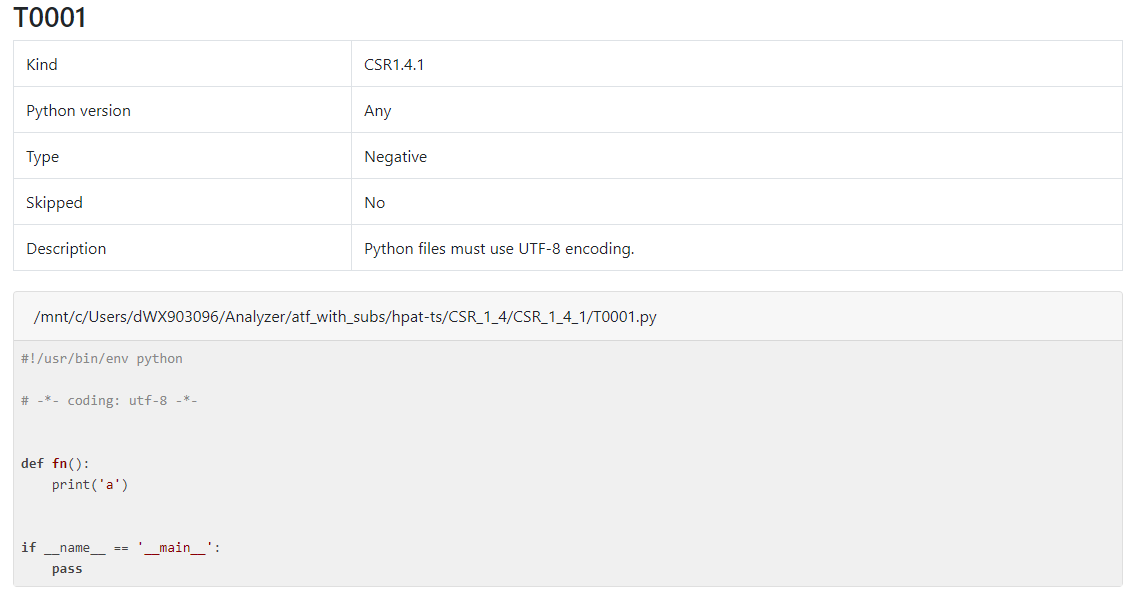
\includegraphics[scale=0.5]{testcase}
  }
  \caption{Тестовый пример}\label{fig:testcase}
\end{figure}


\chapter{Результаты}


\clearpage
